%%%%%%%%%%%%%%%%%%%%%%%%%%%%%%%%%%%%%%%%%%%%%%%%%%%%%%%%%%%%%%%%%%%%%%%%%%%%%%%%%%%%%%%%%%%%%%%%
%
% CS484 Written Question Template
%
% Acknowledgements:
% The original code is written by Prof. James Tompkin (james_tompkin@brown.edu).
% The second version is revised by Prof. Min H. Kim (minhkim@kaist.ac.kr).
%
% This is a LaTeX document. LaTeX is a markup language for producing 
% documents. Your task is to fill out this document, then to compile 
% it into a PDF document. 
%
% 
% TO COMPILE:
% > pdflatex thisfile.tex
%
% If you do not have LaTeX and need a LaTeX distribution:
% - Personal laptops (all common OS): www.latex-project.org/get/
% - We recommend latex compiler miktex (https://miktex.org/) for windows,
%   macTex (http://www.tug.org/mactex/) for macOS users.
%   And TeXstudio(http://www.texstudio.org/) for latex editor.
%   You should install both compiler and editor for editing latex.
%   The another option is Overleaf (https://www.overleaf.com/) which is 
%   an online latex editor.
%
% If you need help with LaTeX, please come to office hours. 
% Or, there is plenty of help online:
% https://en.wikibooks.org/wiki/LaTeX
%
% Good luck!
% Min and the CS484 staff
%
%%%%%%%%%%%%%%%%%%%%%%%%%%%%%%%%%%%%%%%%%%%%%%%%%%%%%%%%%%%%%%%%%%%%%%%%%%%%%%%%%%%%%%%%%%%%%%%%
%
% How to include two graphics on the same line:
% 
% \includegraphics[width=0.49\linewidth]{yourgraphic1.png}
% \includegraphics[width=0.49\linewidth]{yourgraphic2.png}
%
% How to include equations:
%
% \begin{equation}
% y = mx+c
% \end{equation}
% 
%%%%%%%%%%%%%%%%%%%%%%%%%%%%%%%%%%%%%%%%%%%%%%%%%%%%%%%%%%%%%%%%%%%%%%%%%%%%%%%%%%%%%%%%%%%%%%%%

\documentclass[11pt]{article}

\usepackage[english]{babel}
\usepackage[utf8]{inputenc}
\usepackage[colorlinks = true,
linkcolor = blue,
urlcolor  = blue]{hyperref}
\usepackage[a4paper,margin=1.5in]{geometry}
\usepackage{stackengine,graphicx}
\usepackage{fancyhdr}
\setlength{\headheight}{15pt}
\usepackage{microtype}
\usepackage{times}

% From https://ctan.org/pkg/matlab-prettifier
\usepackage[numbered,framed]{matlab-prettifier}

\frenchspacing
\setlength{\parindent}{0cm} % Default is 15pt.
\setlength{\parskip}{0.3cm plus1mm minus1mm}

\pagestyle{fancy}
\fancyhf{}
\lhead{Homework 2 Questions}
\rhead{CS484}
\rfoot{\thepage}

\date{}

\title{\vspace{-1cm}Homework 2 Questions}


\begin{document}
	\maketitle
	\vspace{-3cm}
	\thispagestyle{fancy}
	
	\section*{Instructions}
	\begin{itemize}
		\item 4 questions.
		\item Write code where appropriate.
		\item Feel free to include images or equations.
		\item \textbf{Please use only the space provided and keep the page breaks.} Please do not make new pages, nor remove pages. The document is a template to help grading.
		\item If you really need extra space, please use new pages at the end of the document and refer us to it in your answers.
	\end{itemize}

	\section*{Questions}
	
	\paragraph{Q1:} Explicitly describe image convolution: the input, the transformation, and the output. Why is it useful for computer vision?
	
	%%%%%%%%%%%%%%%%%%%%%%%%%%%%%%%%%%%
	\paragraph{A1:} Your answer here.
	
	Input is an image source that we use to process; and this could be a color image or grayscale image. These images are two dimensional grid data, which has three channel(R,G,B) for color image and single channel(brightness) for grayscale image.

	Without convolution, we need to flatten the image data into one dimensional vector. Usage of convolution makes direct overlay of filter on input image. Convolutional kernel is an square shaped matrix, smaller than the input image. The value of kernel is the weight multiplied in each pixels of input matrix. These products are then summed up to a single value, and we apply this value to the central pixel of output image. We repeat this process for every position in the input image that we can fit the kernel.

The output image is the product of convolution kernel applied to the input image. It has same dimension with the input image, but the outmost pixels disappears, since we cannot apply kernel on the outmost pixels of input image. The output image could emphasize certain features of input image, such as edges, colors, or could apply blur, etc. The effect depends on what kernel we use.

Image convolution is useful in computer vision mainly because we can easily extract features of the input image. We can detect edges, corners, textures by applying different kernel. We could even highlight vertical and horizontal edges in different output. 

Furthermore, we can obtain meaningful effect with convolution, such as noise reduction or image enhancement. Adjustment of brightness and contrast could be performed with convolution, which makes we could analyze the image easier.
	
	
	
	%%%%%%%%%%%%%%%%%%%%%%%%%%%%%%%%%%%
	
	% Please leave the pagebreak
	\pagebreak
	\paragraph{Q2:} What is the difference between convolution and correlation? Construct a scenario which produces a different output between both operations.
	
	
	%%%%%%%%%%%%%%%%%%%%%%%%%%%%%%%%%%%
	\paragraph{A2:} Your answer here.
	
	In convolution, before we apply kernel to input, we flip the kernel horizontally and vertically. Then, we center the kernel over each pixel of input and compute the dot product of kernel and the overlapping area of the input. We put this dot product value in the center pixel  of the input’s area we applied the kernel.

Correlation works same with convolution in making the product and applying the kernel, but the main difference is that we don’t flip the kernel before we apply it on input.

This difference makes convolution commutative, but correlation not commutative.

However because the difference comes from the flipping, if we use symmetric kernel then the result of convolution and correlation could be same.

\begin{lstlisting}[language={python}]
[1, 2, 3]
[4, 5, 6]
[7, 8, 9]
\end{lstlisting}

for this input let's apply 
\begin{lstlisting}[language={python}]
[1, 0, -1]
[-1, 1, -1]
[0, 1, 0]
\end{lstlisting}

for kernel. First, in convolution, we first do horizontal and vertical flip to kernel.
\begin{lstlisting}[language={python}]
[0, 1, 0]
[-1, 1, -1]
[-1, 0, 1]
\end{lstlisting}

Then, the convolution result is 

$(0\times 1) + (1\times2) + (0\times3) + (-1\times4) + (1\times5) + (-1\times6) + (-1\times7) + (0\times8) + (1\times9) = -1$

For correlation, we don't flip the kernel and directly apply it to input.

Then, the correlation result is

$(1\times 1) + (0\times2) + (-1\times3) + (-1\times4) + (1\times5) + (-1\times6) + (0\times7) + (1\times8) + (0\times9) = 1$

which produces different results for convolution and correlation.


	
	%%%%%%%%%%%%%%%%%%%%%%%%%%%%%%%%%%%
	
	% Please leave the pagebreak
	\pagebreak
		\paragraph{Q3:} What is the difference between a high pass filter and a low pass filter in how they are constructed, and what they do to the image? Please provide example kernels and output images.
	
	%%%%%%%%%%%%%%%%%%%%%%%%%%%%%%%%%%%
	\paragraph{A3:} Your answer here.
	
	Low pass filter passes the low frequency value of the input image pass through, while it decreases the high frequency characters of the image.
	This makes the high frequency characters(fine detail, sharpness, noise) of the image decreases, which leads to the blurred image.
	We can create the low pass filter by creating a kernel that emphasizes the central part and supresses the outer part.

	Oppositely, high pass filter pass the high frequency values. It enhances the edges, fine details. It emphasizes the rapid change in the pixel values.
	We can create the high pass filter by creating a kernel that makes the difference between neighbor pixels bigger than the original image was.

	This is the sample low pass filter:
	\begin{lstlisting}[language={python}]
	[1/9, 1/9, 1/9]
	[1/9, 1/9, 1/9]
	[1/9, 1/9, 1/9]
	\end{lstlisting}
	which makes the value of pixel into the sum of decreased value of neighbor pixels.

	This is the sample high pass filter:
	\begin{lstlisting}[language={python}]
	[-1, -1, -1]
	[-1, 8, -1]
	[-1, -1, -1]
	\end{lstlisting}
	
	which subtracts the neighbor pixel values from the center pixel, which makes the pixel difference bigger.

	And these are the output images when we apply the above two kernels in sample image.

	\begin{figure*}[b]
		\centering
		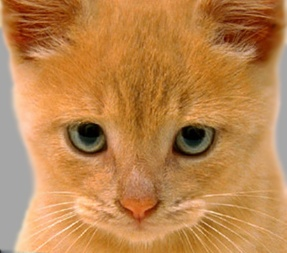
\includegraphics[width=4cm]{/Users/treblocami/Desktop/job/cs484/hw2_2023f/result/lowhighresult/input_image.jpg}
		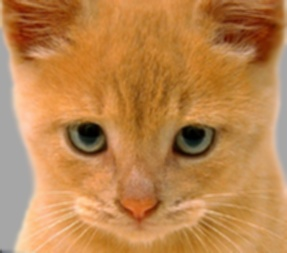
\includegraphics[width=4cm]{/Users/treblocami/Desktop/job/cs484/hw2_2023f/result/lowhighresult/low_pass_image.jpg}
		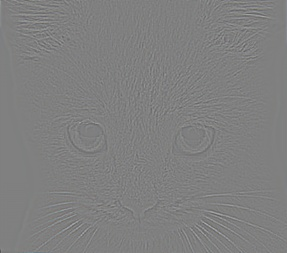
\includegraphics[width=4cm]{/Users/treblocami/Desktop/job/cs484/hw2_2023f/result/lowhighresult/high_pass_image.jpg}
		\caption{From left to right, the input image, low-pass image, and high-pass image.}
	\end{figure*}
	
	%%%%%%%%%%%%%%%%%%%%%%%%%%%%%%%%%%%
	
	% Please leave the pagebreak
	\pagebreak
	\paragraph{Q4:} How does computation time vary with filter sizes from $3\times3$ to $15\times15$ (for all odd and square sizes), and with image sizes from 0.25~MPix to 8~MPix (choose your own intervals)? Measure both using \href{https://docs.opencv.org/4.5.0/d4/d86/group__imgproc__filter.html#ga27c049795ce870216ddfb366086b5a04}{$cv2.filter2D()$} to produce a matrix of values. Use the \href{https://docs.opencv.org/4.5.3/da/d54/group__imgproc__transform.html#ga47a974309e9102f5f08231edc7e7529d}{$cv2.resize()$} function to vary the size of an image.
	Use an appropriate \href{https://jakevdp.github.io/PythonDataScienceHandbook/04.12-three-dimensional-plotting.html#Three-dimensional-Contour-Plots}{3D charting function} to plot your matrix of results, such as $plot\_surface()$ or $contour3D$.
	
	Do the results match your expectation given the number of multiply and add operations in convolution?
	
	See RISDance.jpg in the attached file.
	
	%%%%%%%%%%%%%%%%%%%%%%%%%%%%%%%%%%%
	\paragraph{A4:} Your answer here.

	Computation time proportionally increased as the image size increased. However, it didn't increased with filter size.
	Oppositely, it showed the largest computation time when filter size = 11, and decreased as the filter gets bigger. We could notice it in [figure 2].

	To compare it to the actual multiplication and addition numbers, I measured the computation time with $my\_filter2D()$, which is composed with actuall multiplication of kernel and input.
	In this case, the computation time was retained even though the filter size increased. Also, it increased proportionally to the image size, which is the same as $cv2.filter2D()$.

	The second graph matches with the actual expectation based on the number of multiplication and addition, because the actual operation numbers doesn't increase when the filter size increases.

	\begin{figure*}[b]
	\centering
	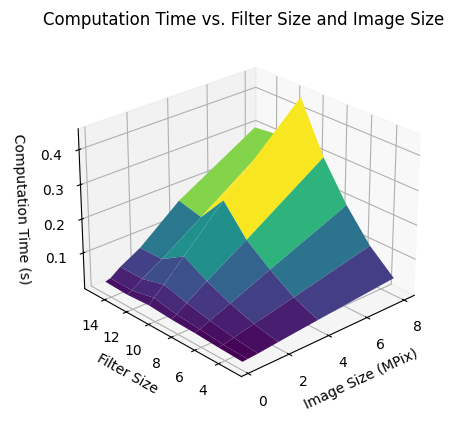
\includegraphics[width=6cm]{/Users/treblocami/Desktop/job/cs484/hw2_2023f/questions/graph6.png}
	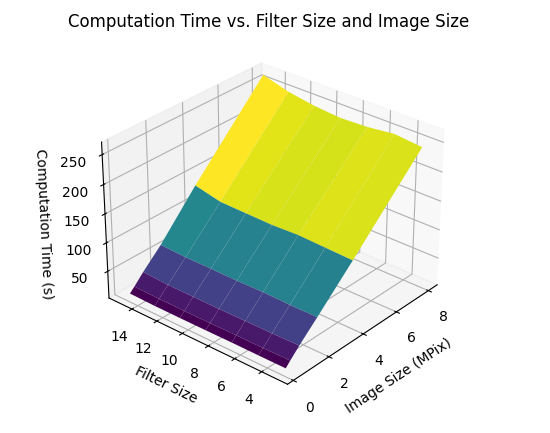
\includegraphics[width=7cm]{/Users/treblocami/Desktop/job/cs484/hw2_2023f/questions/graph7.png}
	\caption{Left: $cv2.filter2D()$, Right: $my\_filter2D()$}
	\end{figure*}
	%%%%%%%%%%%%%%%%%%%%%%%%%%%%%%%%%%%
	
	
	% If you really need extra space, uncomment here and use extra pages after the last question.
	% Please refer here in your original answer. Thanks!
	%\pagebreak
	%\paragraph{AX.X Continued:} Your answer continued here.
	
	
	
\end{document}